% XCircuit output "block.tex" for LaTeX input from block.eps
\def\putbox#1#2#3#4{\makebox[0in][l]{\makebox[#1][l]{}\raisebox{\baselineskip}[0in][0in]{\raisebox{#2}[0in][0in]{\scalebox{#3}{#4}}}}}
\def\rightbox#1{\makebox[0in][r]{#1}}
\def\centbox#1{\makebox[0in]{#1}}
\def\topbox#1{\raisebox{-0.60\baselineskip}[0in][0in]{#1}}
\def\midbox#1{\raisebox{-0.20\baselineskip}[0in][0in]{#1}}
   \scalebox{1}{
   \normalsize
   \parbox{15.0625in}{
   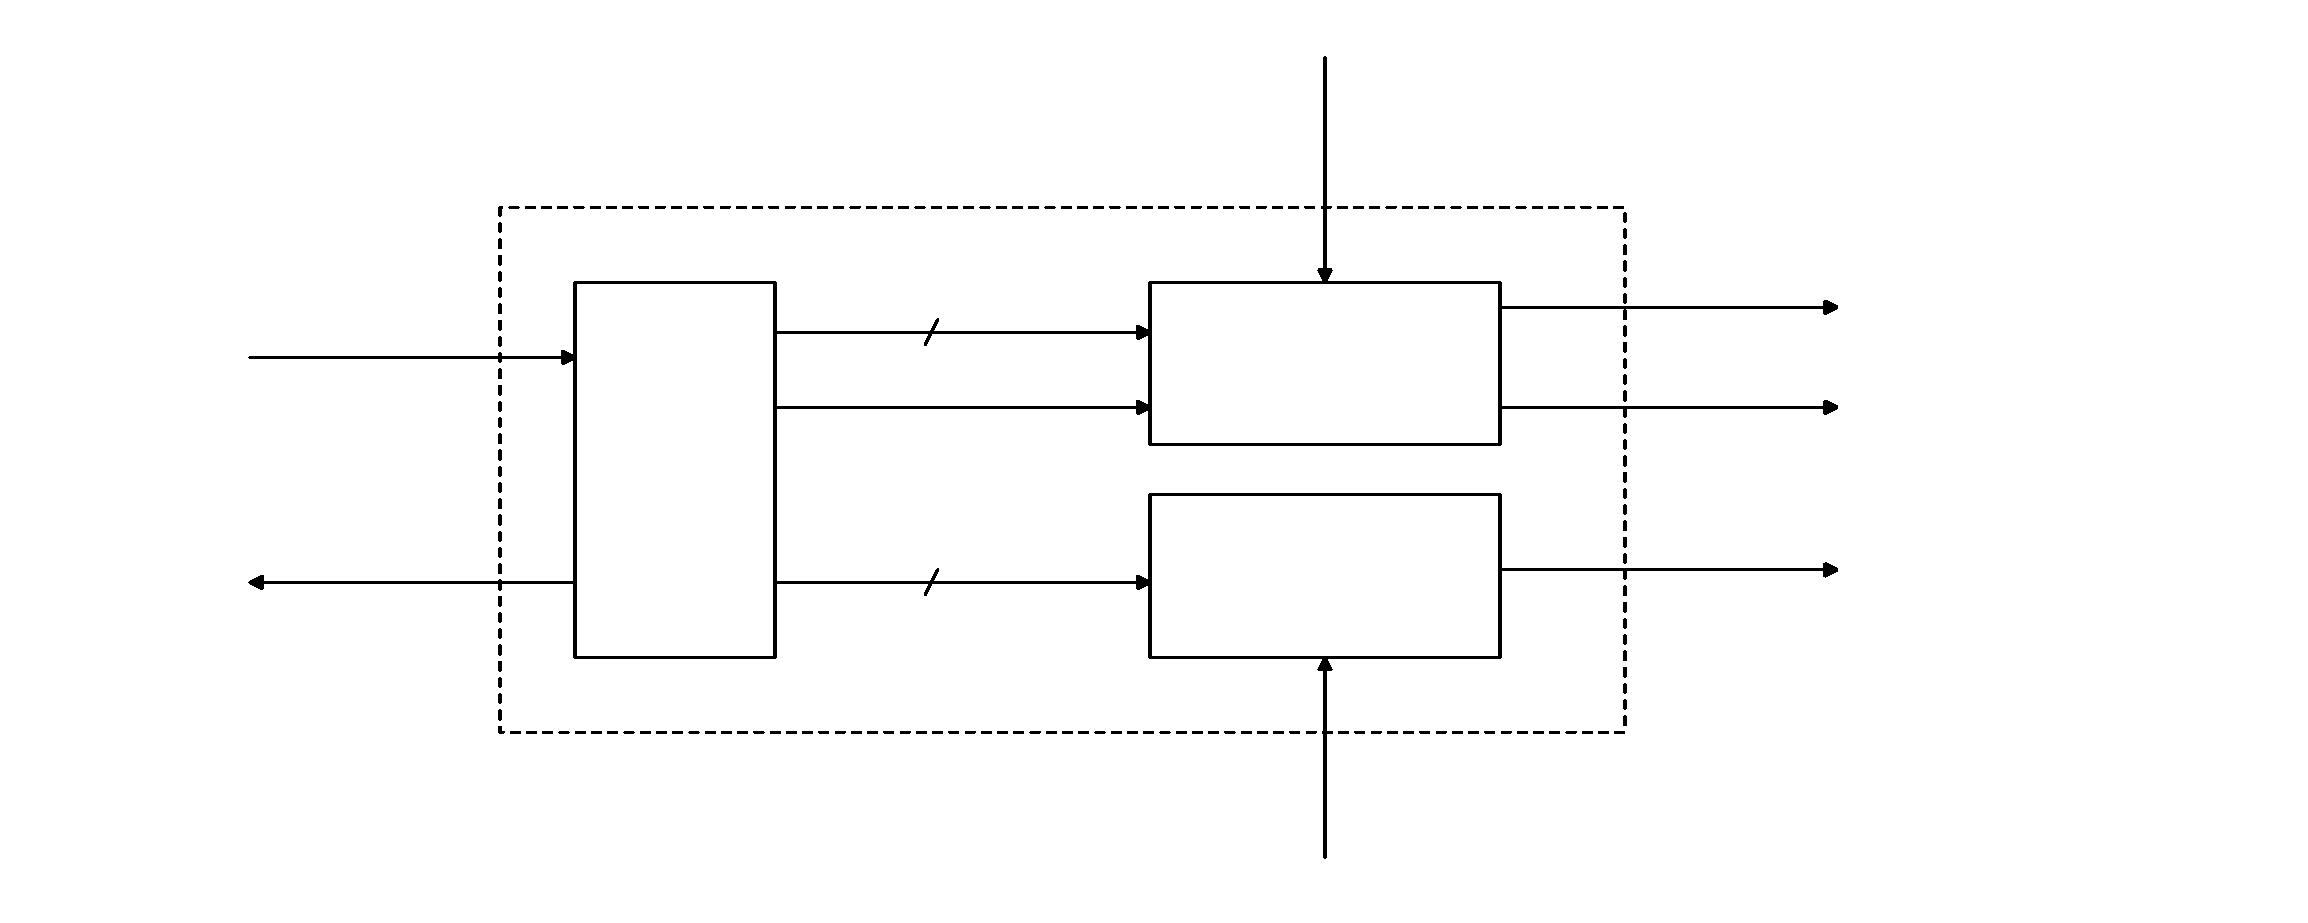
\includegraphics[scale=1]{block.eps}\\
   % translate x=1504 y=628 scale 0.38
   \putbox{3.31in}{4.74in}{1.20}{TEU Debug Unit}%
   \putbox{0.14in}{3.83in}{1.20}{ccu\_to\_teu\_debug\_unit\_command}%
   \putbox{0.06in}{2.33in}{1.20}{teu\_debug\_unit\_to\_ccu\_response}%
   \putbox{4.05in}{2.63in}{1.20}{\shortstack[lb]{CCU\\interface\\unit}}%\
   \putbox{8.31in}{5.74in}{1.20}{PC, valid}%
   \putbox{7.39in}{0.08in}{1.20}{mem adress, valid, read/write}%
   \putbox{11.22in}{4.16in}{1.20}{teu\_debug\_unit\_to\_stream\_corrector\_bp}%
   \putbox{11.22in}{3.49in}{1.20}{teu\_debug\_unit\_to\_stream\_corrector\_intr}%
   \putbox{11.22in}{2.41in}{1.20}{teu\_debug\_unit\_to\_stream\_corrector\_wp}%
   \putbox{8.12in}{3.4in}{1.20}{\shortstack[lb]{breakpoint and\\interrupt unit}}%
   \putbox{8.07in}{2.11in}{1.20}{watchpoint unit}%
   \putbox{5.31in}{3.99in}{1.20}{4 breakpoint signals}%
   \putbox{5.56in}{3.49in}{1.20}{interrupt signal}%
   \putbox{5.31in}{2.33in}{1.20}{4 watchpoint signals}%
   } % close 'parbox'
   } % close 'scalebox'
   \vspace{-\baselineskip} % this is not necessary, but looks better
